\documentclass[10pt,letterpaper]{article}

\usepackage{hyperref}
\usepackage{cogsci}
\usepackage{pslatex}
\usepackage{apacite}
\usepackage{graphicx}
\usepackage{todonotes}
\usepackage{caption}
\usepackage{subcaption}

\title{Extremely costly intensifiers are stronger than quite costly ones: a case of non-arbitrary word meanings.}
 
\author{{\large \bf Erin Bennett (erindb@stanford.edu)} \\
  Department of Psychology, 450 Serra Mall , Stanford, CA 94305
  \AND {\large \bf Noah Goodman (ngoodman@stanford.edu)} \\
  Department of Psychology, 450 Serra Mall , Stanford, CA 94305}


\begin{document}

\maketitle


\begin{abstract}
%Intensifiers of scalar adjectives might derive the degree of their meaning from their cost.
%We show that surprisal and syllable length, two different construals of the cost of an intensifier, both independently predict estimates of degree.
%We further show that when an intensifier is frequently repeated within a ``non-standard dialect of English'' (i.e. when we manipulate the surprisal of an intensifier), its inferred degree is consequently lower.

\todo[inline]{abstract}

\textbf{Keywords:} 
intensifiers; degree adverbs; scalar adjectives; pragmatics; m-implicature
\end{abstract}


\section{Introduction}

\todo[inline]{is there a nice saussure quote to summarize the arbitrariness position?}

Where do words get their meanings? For instance, why is an ``extremely good paper'' better than a ``quite good paper''? The traditional answer \cite{saussure} is that different meanings have been arbitrarily and conventionally assigned to the different word forms.
In this paper we explore adjectival intensifiers, like ``extremely'' and ``quite'', as a case study in which to empirically explore the relationship of meaning to form.
Based on a previous theory of the semantics of scalar adjectives we hypothesize that the interpreted meanings of intensifiers are (at least partly) non-arbitrary, and instead are determined by their production (or comprehension) cost. 
We show in three experiments that the meanings of english intensifiers are predictable from their costs, and are sensitive to manipulation of cost.
These results are consistent with the small but growing literature arguing that word meanings are not fully arbitrary, but instead are constrained by non-semantic features of the word. 

\todo[inline]{a paragraph here unpacking the question of word-meaning mapping. start with what saussure said about signs. this suggests that meaning is purely the result of historical accident. certainly a lot of meaning for a lot of words must be arbitrary -- without convention there is no language. mention the recent work on modeling language evolution. however, there is some evidence that meaning is not entirely arbitrary: kiki-boba stuff, and maybe molly's results. to resolve this tension we will need more, and more quantitative case-studies where we can explore the extent of non-arbitrary factors.}

\todo[inline]{next a paragraph talking about adjectives and intensifiers. scalar adjs probably have a threshold semantics (cite kennedy) and the threshold is set in a pragmatic way that depends on context. lassiter and goodman give a formal model of setting the threshold. given this story about adjectives, what could intensifiers do? it's possible to posit a complex semantic mechanism by which they grab and alter the threshold which has been set for the adjective (as if they weren't there). however a more parsimonious hypothesis is that they don't have any semantic effect--instead their ``meaning'' is a result of their cost and the impact this has on pragmatic inference. possibly stick in the model result (without model details) to show that this really would be expected to happen?}

\todo[inline]{perhaps a short paragraph drawing out the implication of this story: asking whether the word-form to lexical-semantics mapping is arbitrary is not the right question, because pragmatics is inextricably part of the process of interpretation, and pragmatics is sensitive to additional factors which are not purely phonetic or lexical semantic.}

\todo[inline]{note: can we explain why bad can be used to mean very good?}

\todo[inline]{finally a very brief paragraph giving the roadmap of our experiments.}

Intensifiers, like ``extremely'' and ``quite'', are adverbs that modify scalar adjectives to change the degree of the resulting adjective phrase.
Scalar adjectives have been modeled as having implicit thresholds that need to be inferred from the context, and intensifiers seem to raise that threshold, e.g. the threshold above which people are ``extremely tall'' is higher than the threshold above which people are ``tall''.
Some intensifiers seem to change this threshold more than others, and the extent to which they do might be influenced by online or conventionalized M-implicature.




%then unpack this argument in a couple paragraphs (including the fancy saussure mention) and motivate the experiments. connect briefly to the few other cases of non-arbitrary meanings.

%part of this unpacking should set up the idea that meanings of intensifiers could depend non-arbitrarily on their cost (perhaps by mentioning M-implicature?), and the notion that cost should depend on frequency, articulation complexity, and possibly other things.


%form / meaning / and meaning-setting information -- distinguish the three in discussion.

%for the intro, i think we will want to explore a bit the question of arbitrariness of word meaning: http://en.wikipedia.org/wiki/Sign_(linguistics) . it's good to start with and example and with a big picture question. so it might be something like: why is an "extremely good paper" better than a "quite good paper"? the traditional answer is that these words simply have different meanings which have been arbitrarily and conventionally assigned to their forms. in this paper we explore the hypothesis that the meanings of intensifiers are at least partly non-arbitrary, but instead are determined by aspects of their production (or comprehension) cost. then unpack this argument in a couple paragraphs (including the fancy saussure mention) and motivate the experiments. connect briefly to the few other cases of non-arbitrary meanings.

%part of this unpacking should set up the idea that meanings of intensifiers could depend non-arbitrarily on their cost (perhaps by mentioning M-implicature?), and the notion that cost should depend on frequency, articulation complexity, and possibly other things.


%let's use "frequency" or "inverse frequency" where possible, instead of surprisal (since that is more technical).

%\todo[inline]{complexity, bouba/kiki, m-implicature, ...}

% Intensifiers, for example ``extremely'' or ``very'', are adverbs that modify scalar adjectives to increase their degree.
% We argue that the meanings of intensifiers are likely not just arbitrarily paired with their words, but that some intensifiers have stronger meanings as a result of the cost it takes to utter them.
% 
% The specific meanings that scalar adjectives take can be inferred pragmatically from context (cite).
% The specific meaning of an intensifier might be inferred from context in a similar way.
% %Though many aspects of an intensifier's meaning, and its affinity to be paired with certain adjectives over others, are probably conventionalized, much of the meaning 
% 
% Longer and more suprising intensifiers are more costly to utter, and so in this paper we look at how suprisal and syllable length relate to the strengths of different intensifiers.
% We find that longer, more surprising intensifiers tend to have stronger meanings.
% 
% The fact that the surprisal of an intensifier might influence its strength means that as the frequency and therefore the surprisal of an intensifier changes over time in a dialect, the strength will also change.
% An interesting consequence \todo{which i think we have evidence for... cite?} is that new intensifiers might continually need to be created to replace old, faded ones.
% We show that intensifiers are quite malleable and that people can learn that within a new ``version of English'' a particular intensifier is used much more frequently than in standard English, and they consequently infer a weaker meaning for the overused word.

%The longer and more unusual a word is, the less easy it would be to say or to understand.
%These words are numerous in English, are relatively easy to coin, and the use of one intensifier over another (e.g. ``wicked fun'' rather than ``totally fun'') often suggests membership in a particular social group or dialect.
%We provide evidence for the claim that intensifiers' meanings are derived, at least in part, from pragmatic inference using their cost.
%The cost of uttering an intensifier, which we approximate using syllable length and also surprisals calculated from corpus frequencies from Google Ngrams, largely predicts the degree people will ascribe to it.
%When we create an imaginary dialect of English in which a particular intensifier is overused, we find that that intensifier is inferred to have a weeker meaning than when it is not repeated.
%Scalar adjectives, free semantic threshold variables, and m-implicature. Language change.
% To explore the hypothesis that the meanings of intensifiers are a function of their cost, we first wanted to see whether surprisal and syllable length (two different ways of measuring the cost of a word) were even correlated with the meanings of intensifiers. We ran two experiments: one with a free response dependent measure and one with a ranking dependent measure.

\section{Experiment 1}

To explore the hypothesis that the interpretations of intensifiers are a function of their cost, we first wanted to see whether two possible ways of measuring the cost of a word, frequency (rarer words are probably more costly) and syllable length, were related to the interpretations of intensifiers.

\subsection{Method\footnote{The full experiment can be found at \url{http://web.stanford.edu/~erindb/degree-adverbs/experiments/exp5_2014-12-01/exp5.html}}}

40 participants with US IP addresses participated in our Experiment 1 on Amazon's Mechanical Turk.

We asked participants to give us judgements of prices based on a person's description of an object that included an intensifier (Figure~\ref{exp1-q}).
There were three categories of objects (\emph{laptop}, \emph{watch}, and \emph{coffee maker}) and 40 intensifiers (see Table~\ref{exp1-intensifiers}).
We chose intensifiers that have a wide range of frequencies and excluded intensifiers that are either more commonly used to signal affect than to signal degree (e.g. ``depressingly expensive'' might indicate a degree, but it definitely indicates affect) or are ambiguous between other parts of speech (e.g. ``super'' can be used as an intensifier, as in ``super expensive'', but it can also be used as an adjective, as in ``super hero'').
Each particpant gave price judgements for every intensifier-category pairing in randomized order, for a total of 120 price judgements.
We chose the domain of price and used only the adjective ``expensive'', because price gave a quantitative scale on which to measure the different intensifers and because we thought participants would have similar enough experience with the distributions over prices for these objects.
% come to think of it, we chose those exact objects because we thought they might have bimodal priors. possibly in future experiments where the analysis would be easier if people had the same distribution as one another, we should go to something that people purchase more frequently with less ambiguity about ``what kind''... like milk, or shampoo...?

\begin{figure}[ht]
\begin{center}
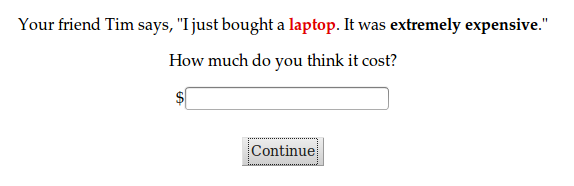
\includegraphics[width=0.4\textwidth]{analysis_files_for_writeup/images/exp1-q.png}
\end{center}
\caption{Screenshot from Experiment 1 target question.} 
\label{exp1-q}
\end{figure}

\begin{table}[ht]
 \begin{center}
  \caption{Intensifiers from Experiment 1, number of occurences in Google Web 1T 5grams corpus, and number of syllables.}
  \label{exp1-intensifiers}
  \begin{tabular}{ccc}
   \hline
   ngram & frequency & syllables \\
    \hline
    surpassingly & 11156 & 4 \\
    colossally & 11167 & 4 \\
    terrifically & 62292 & 4 \\
    frightfully & 65389 & 3 \\
    astoundingly & 73041 & 4 \\
    phenomenally & 120769 & 5 \\
    uncommonly & 135747 & 4 \\
    outrageously & 240010 & 4 \\
    fantastically & 250989 & 4 \\
    mightily & 252135 & 3 \\
    supremely & 296134 & 3 \\
    insanely & 359644 & 3 \\
    strikingly & 480417 & 3 \\
    acutely & 493931 & 3 \\
    awfully & 651519 & 3 \\
    decidedly & 817806 & 4 \\
    excessively & 877280 & 4 \\
    extraordinarily & 900456 & 6 \\
    exceedingly & 977435 & 4 \\
    intensely & 1084765 & 3 \\
    markedly & 1213704 & 3 \\
    amazingly & 1384225 & 4 \\
    radically & 1414254 & 3 \\
    unusually & 1583939 & 4 \\
    remarkably & 1902493 & 4 \\
    terribly & 1906059 & 3 \\
    exceptionally & 2054231 & 5 \\
    desperately & 2139968 & 3 \\
    utterly & 2507480 & 3 \\
    notably & 3141835 & 3 \\
    incredibly & 4416030 & 4 \\
    seriously & 12570333 & 4 \\
    truly & 19778608 & 2 \\
    significantly & 19939125 & 5 \\
    totally & 20950052 & 3 \\
    extremely & 21862963 & 3 \\
    particularly & 41066217 & 5 \\
    quite & 55269390 & 1 \\
    especially & 55397873 & 4 \\
    very & 292897993 & 2
  \end{tabular}
 \end{center}
\end{table}

\subsubsection{Corpus Methods}
%maybe have this a separate section? maybe not?

In order to measure the cost associated with different intensifiers, we collected their length in syllables and their frequencies (Table~\ref{exp1-intensifiers}).
The frequencies were collected from the Google Web 1T 5-grams database \cite{web1t5gram}\footnote{
We also ran the same analyses on frequency information collected from the Google Books American Ngrams Corpus \cite{books2011} as well, and found similar results.

In addition, we did the same using the bigram frequencies of ``\emph{[intensifer]} expensive'' rather than the unigram frequencies of the intensifiers alone. These data were much more sparse. For bigrams, we found no significant effects of surprisal using the books database and a negative effect using the web database.
}
The syllable lenths of our intensifiers and the surprisals were correlated, but not strongly so (r = 0.2648144).

\subsection{Results and Discussion}

If the meaning of an intensifier is stronger for higher cost intensifiers, we would expect to find that as frequency decreases and length in syllables increases, the prices participants give will also increase. We find that this is the case.

\begin{figure}[ht]
\begin{center}
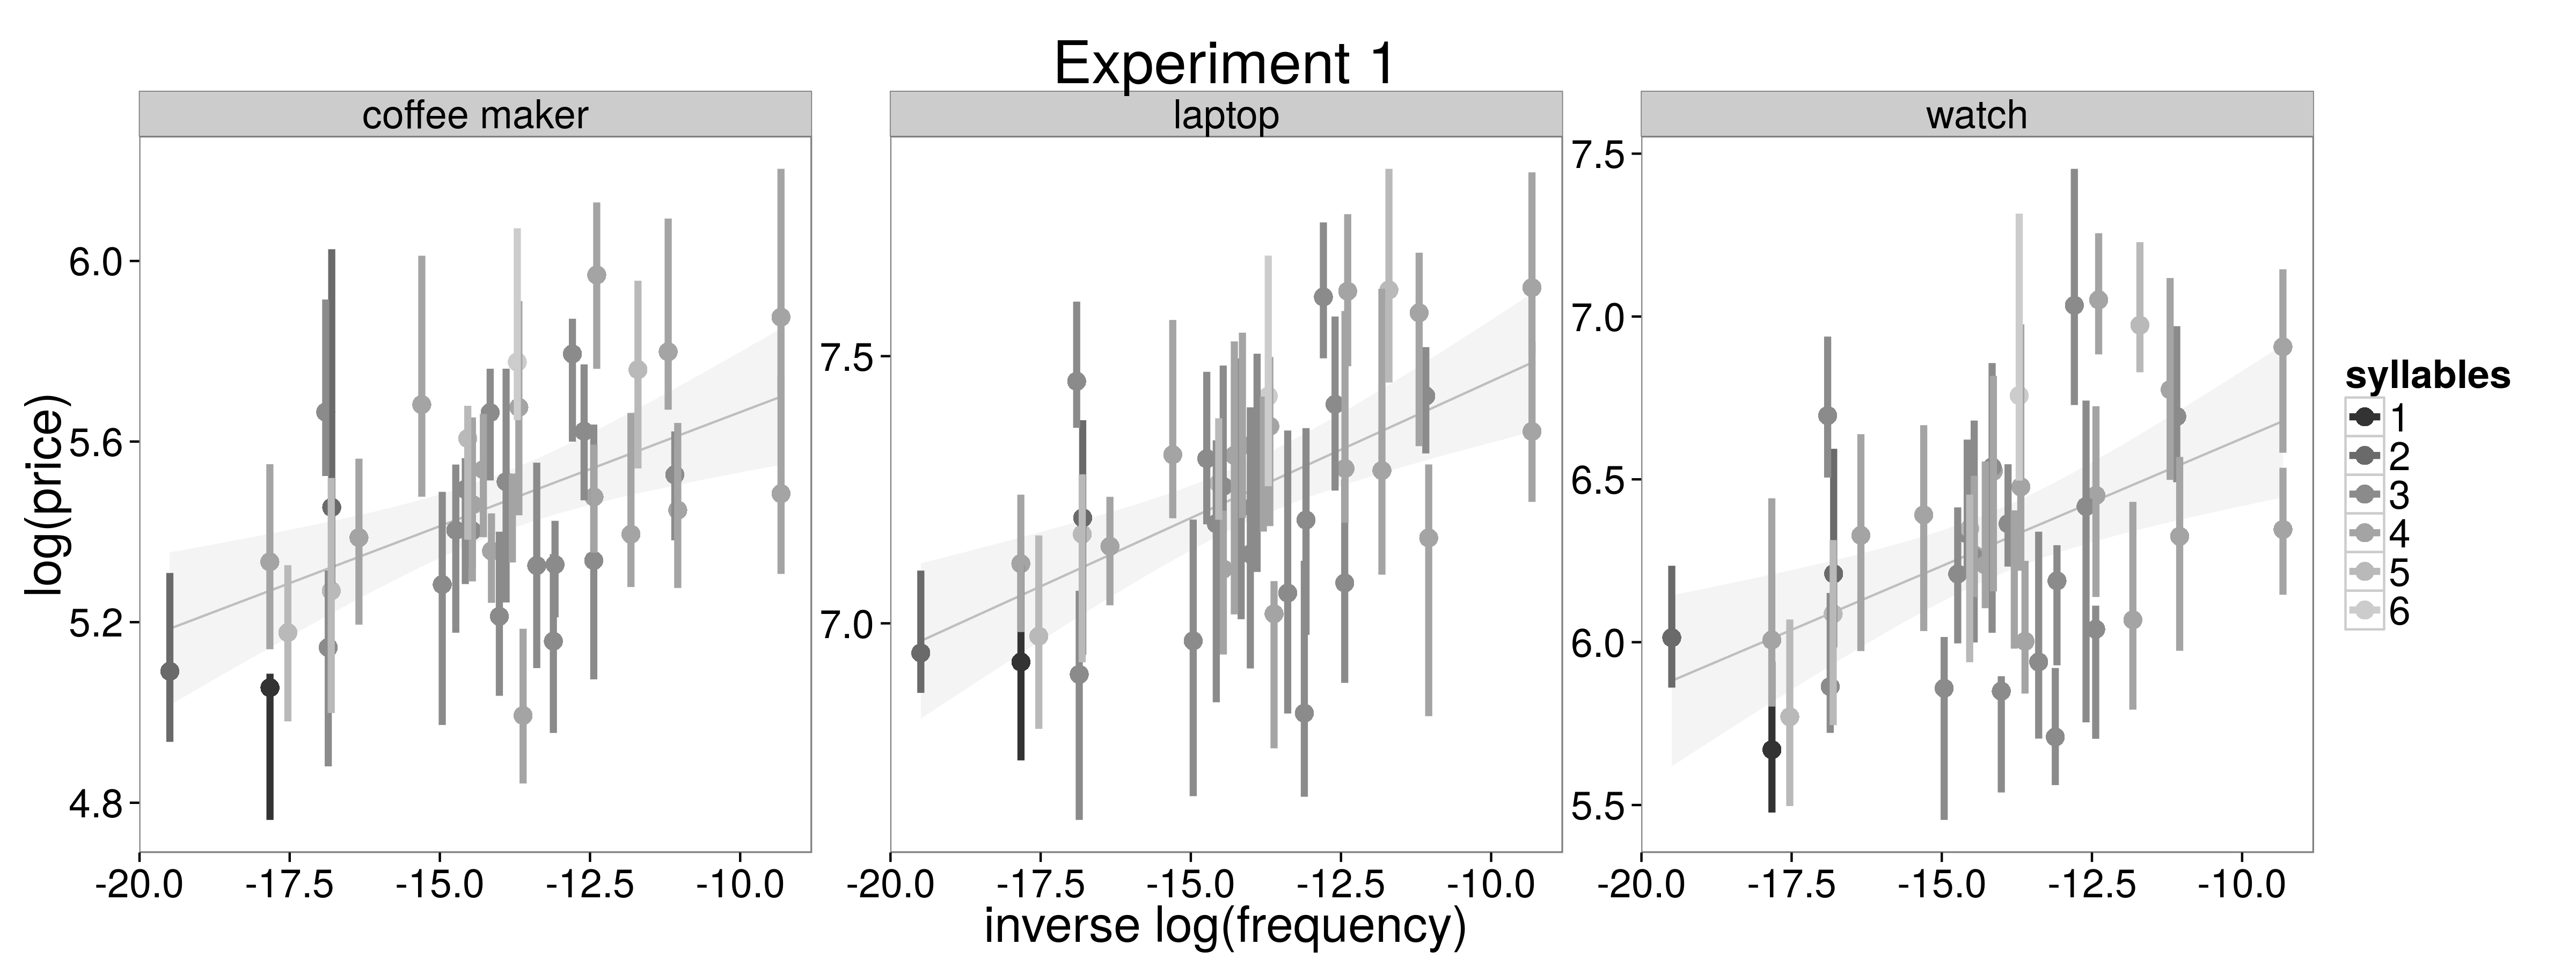
\includegraphics[width=0.48\textwidth]{analysis_files_for_writeup/images/exp1-plot.png}
\end{center}
\caption{Results of Experiment 1. As surprisal and length in syllables increase, participants' free response prices increased.} 
\label{exp1-plot}
\end{figure}

In a linear mixed effects regression with centered fixed effects of syllables and surprisal and their interaction and random intercepts and slopes for syllables and surprisal for both participant and object, we found significant main effects of surprisal (estimate=0.054, p=0.012) and syllable length  (estimate=0.093, p=0.0041) as well as a significant interaction (estimate=0.019, p=0.00018).
%anything more complicated won't converge

The interaction suggests that the function from surprisal and frequencies to cost might be multiplicative.

So intensifiers that are more surprising and longer (and therefore are more costly to utter) also tend to be interpreted as having stronger meanings.

\todo[inline]{make a big deal}

\section{Experiment 2}

In Experiment 2, we replicated our finding from Experiment 1 using a different dependent measure which we expect to be more sensitive to small differences in meaning and an extension to other adjectival scales.

\subsection{Method\footnote{The full experiment can be found at \url{http://web.stanford.edu/~erindb/degree-adverbs/experiments/exp4/exp4.html}}}

30 participants with US IP addresses participated in our Experiment 2 on Amazon's Mechanical Turk.

Because arranging all 40 intensifiers on a computer screen would be difficult for participants, we divided the 40 intensifiers from Experiment 1 into four lists of 10 intensifiers each (Table~\ref{exp2-intensifiers}).
Each list was randomly paired with one of four adjectives (``old'', ``expensive'', ``beautiful'', and ``tall'').
For each adjective-list pairing, participants were shown every combination of the 10 intensifiers and the one adjective on the left side of the screen.
They were asked to move the adjective phrases from the left to the right side of the screen, reordering the phrases from the lowest to the highest degree (Figure~\ref{exp2-q}).
Each participant did four trials of this process, seeing all four lists and all four adjectives.
The pairings between list and adjective were randomized between participants.
The division of the intensifiers into lists of 10 was constant, i.e. the same 10 intensifiers were always shown together.

\begin{figure}[ht]
\begin{center}
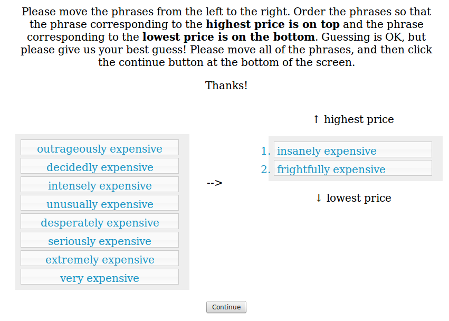
\includegraphics[width=0.4\textwidth]{analysis_files_for_writeup/images/exp2-q.png}
\end{center}
\caption{Screenshot from Experiment 2 target question.} 
\label{exp2-q}
\end{figure}

\begin{table}[ht]
\begin{center} 
\caption{Intensifier Lists from Experiment 2: Rankings.} 
\label{exp2-intensifiers} 
\vskip 0.12in
\begin{tabular}{cccc} 
\hline
List A    &  List B & List C & List D \\
\hline
surpassingly & colossally & terrifically & frightfully \\
astoundingly & phenomenally & uncommonly & outrageously \\
fantastically & mightily & supremely & insanely \\
strikingly & acutely & awfully & decidedly \\
excessively & extraordinarily & exceedingly & intensely \\
markedly & amazingly & radically & unusually \\
remarkably & terribly & exceptionally & desperately \\
utterly & notably & incredibly & seriously \\
truly & significantly & totally & extremely \\
particularly & quite & especially & very
\end{tabular}
\end{center}
\end{table}

\subsection{Results and Discussion}

Within each intensifier list, we ran a regression using centered syllable length and surprisal to predict the ranking that participants gave the adjective phrase (the highest ranked adjective phrase in a trial got a ranking of 10, the lowest ranked adjective phrase got a ranking of 1).
For the two lists with a large enough range of syllable lengths, we fully replicated our results from Experiment 1.
For the two lists with smaller syllable ranges, we replicated the main effect of surprisal, but found different effects of syllable length.
Results were very similar across the four different adjectives.

\begin{figure}[ht]
\begin{center}

\includegraphics[width=0.48\textwidth]{analysis_files_for_writeup/images/exp2-plot.png}
\end{center}
\caption{Results of Experiment 2. As surprisal and length in syllables increase, participants' rankings increased.} 
\label{exp2-plot}
\end{figure}

For the lists A and B, which each contained five different lengths of syllables, we found significant main effects of surprisal (list A: estimate=0.45, p=1.1e-7; list B: estimate=0.45, p=1.9e-15) and syllable length (list A: estimate=0.87, p=0.0051; list B: estimate=1.3, p=2e-16) and a significant interaction (list A: estimate=0.25, p=0.034; list B: estimate=0.20, p=1.0e-6), as in Experiment 1.
For lists C and D, which had only three different syllable lengths, we found main effects of surprisal (list C: estimate=0.36, p=3.3e-5; list D: estimate=0.46, p=9.6e-6), but no positive effect of syllable length and no positive interaction.
For list C, there was no main effect of syllable length (p=0.49) and a negative interaction (estimate=-0.52, p=0.0045). For list D, there was a negative main effect of syllable length (estimate=-1.4, p=4.5e-6) and a negative interaction (estimate=-0.23, p=0.024).

Overall, we again found that participants assign stronger interpretations to intensifiers with lower frequencies and higher syllable lengths.

\todo[inline]{more about this?}

The relationship between frequency and interpretation might be causal, and the causal direction might be that the rarity of the word causes it to be costly to use and therefore to correspond to a stronger meaning, as in our hypothesis.
However, the causal direction could also be the opposite.
Perhaps the fact that an intensifier has a stronger meaning (which it may have gotten completely arbitrarily) causes it to be used only in extreme and unusual circumstances.
Since these circumstances rarely occur, the strong intensifier will rarely be said\footnote{This assumes that people talk about things about as frequently as they happen, which might not be the case... Isn't someone here working on how representative the internet is of what actually happens, and super rare things have an inflated presence on the web? Which is kind of evidence that people talk about extreme things more than they actually happen.}.
This story seems possible, but would not be able to account for why syllable length above and beyond surprisal would predict stronger meanings in most of our experimental conditions.

\section{Experiment 3}

We test the direction of this relationship more directly in Experiment 3 by exposing participants to an imaginary dialect and manipulating the frequency with which intensifiers occur.
If people use the frequency of an intensifier in order to interpret it, and the rarity of an intensifier causes its interpreation to be stronger, then changing and intensifier's frequency should change its interpretation. b

\subsection{Method\footnote{The full experiment can be found at \url{http://web.stanford.edu/~erindb/degree-adverbs/experiments/exp8/exp8.html}}}

%expt 3: describe the training story a bit more: length, content, etc.

20 participants with US IP addresses participated in our Experiment 3 on Amazon's Mechanical Turk.

We trained participants on a dialect that used one of two short intensifiers, ``truly'' and ``very'' much more frequently than in standard English.
The speaker of this dialect, Jim, was a character in a comic who lived ``across the country'' in a town with ``a distinct way of speaking''.
We showed participants a 9-panel comic in which Jim told his visiting cousin about a big storm that had knocked down a tree into his kitchen and about a friend's child who had taken part of the tree home with him (Figure~\ref{exp3-story}).
Jim said 294 words in the training story, 22 of which were the target intensifier (either ``truly'' or ``very'', varied between participants).

\begin{figure}
        \centering
        \begin{subfigure}[b]{0.45\textwidth}
                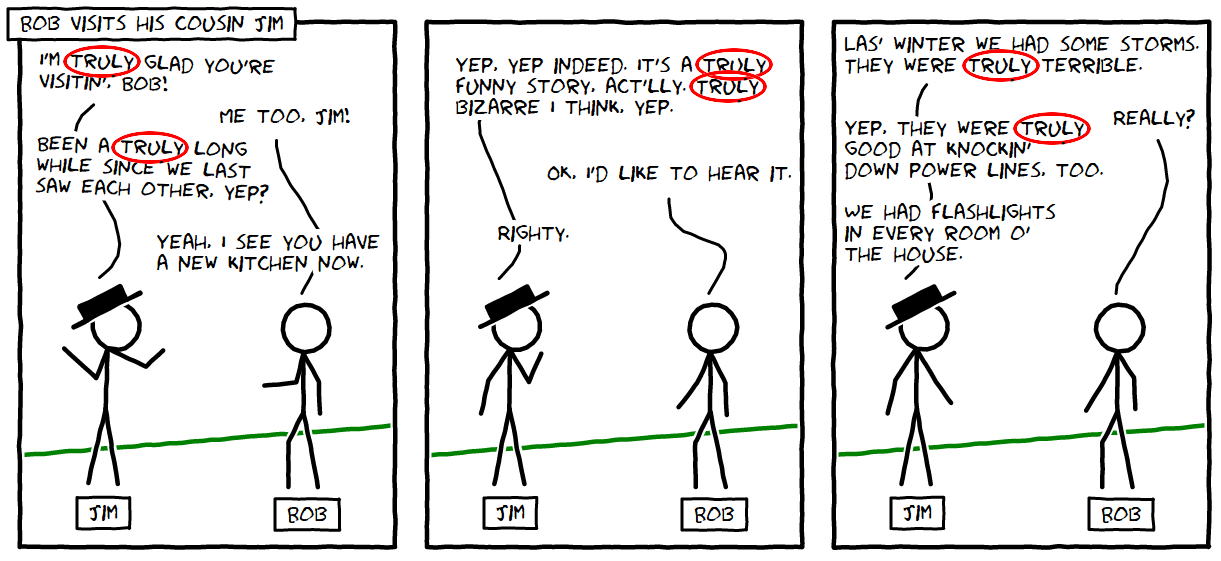
\includegraphics[width=\textwidth]{analysis_files_for_writeup/images/story1_truly_circles.png}
        \end{subfigure}%
        
        \begin{subfigure}[b]{0.45\textwidth}
                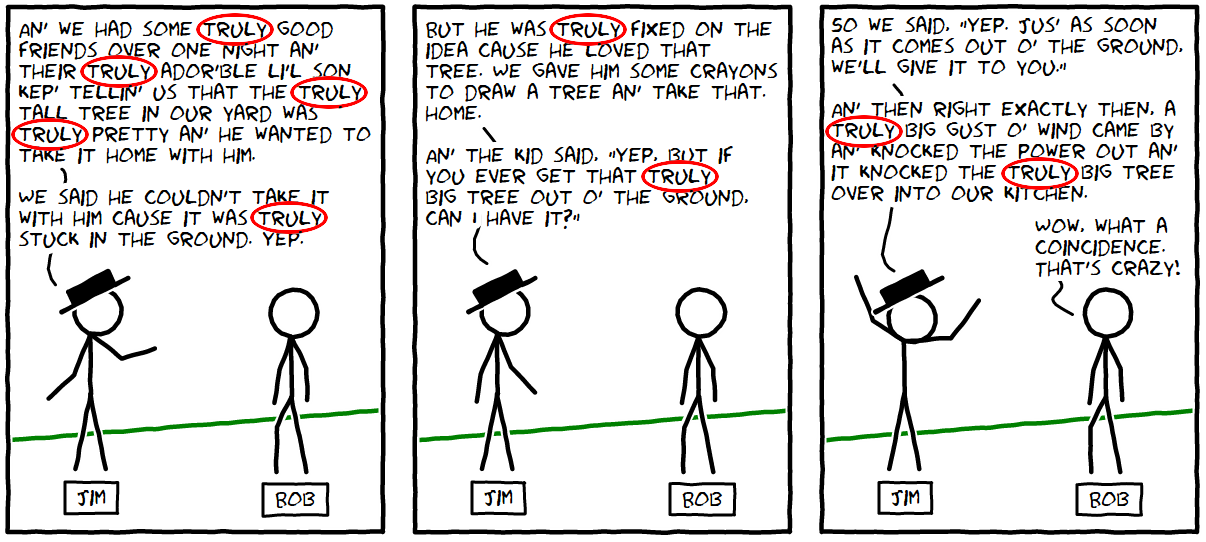
\includegraphics[width=\textwidth]{analysis_files_for_writeup/images/story2_truly_circles.png}
        \end{subfigure}
        
        \begin{subfigure}[b]{0.45\textwidth}
                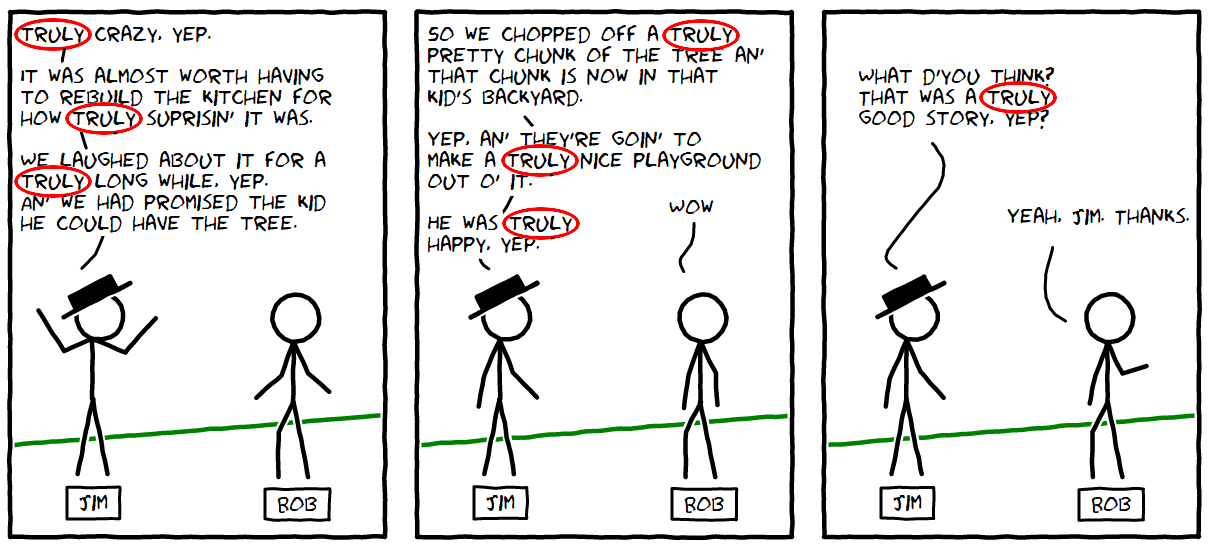
\includegraphics[width=\textwidth]{analysis_files_for_writeup/images/story3_truly_circles.png}
        \end{subfigure}
        \caption{Full training story comic for Experiment 3, target intensifier ``truly'' is repeated 22 times, control target ``very'' is not used.}\label{exp3-story}
\end{figure}

After the training story, participants were immediately shown a final panel, where Jim described a coffee maker he recently purchased, but part of his utterance was missing (Figure~\ref{exp3-q}).
Participants were asked to give a price judgement for each of three different possible utterances: the two intensifiers, and the bare ``expensive'' form.
One of these intensifiers was the target intensifier which occured in the training story, and one intensifier was the control intensifier which did not occur in the story.
So for each of the two intensifiers, some participants gave ratings for it as a target intensifier and some participants gave ratings for it as a control intensifier.

% We looked at two short intensifiers of equal length: ``truly'' and ``very''. In our two conditions (varied between participants), each intensifier was either the target or the control. In a comic-style training story, the target intensifier was repeated 22 times by a speaker who lived ``across the country'' and had ``a distinct way of speaking.'' The control intensifier was not used by the speaker in the story.
% 
% To guage whether participants had learned that the speaker's use of the target intensifier was unusually high, we asked participants how many times in the next 1000 words they thought the speaker would use the control word, the target word, and another word that had been frequently repeated.
% 
% To determine what strength participants inferred for the target and control intensifiers, we gave participants a final panel of the comic where the speaker described a new coffee maker he bought (Fig~\ref{exp3-q}). We asked participants to guess the price of the coffee maker given different possible descriptions the speaker could have used.

\begin{figure}[ht]
\begin{center}
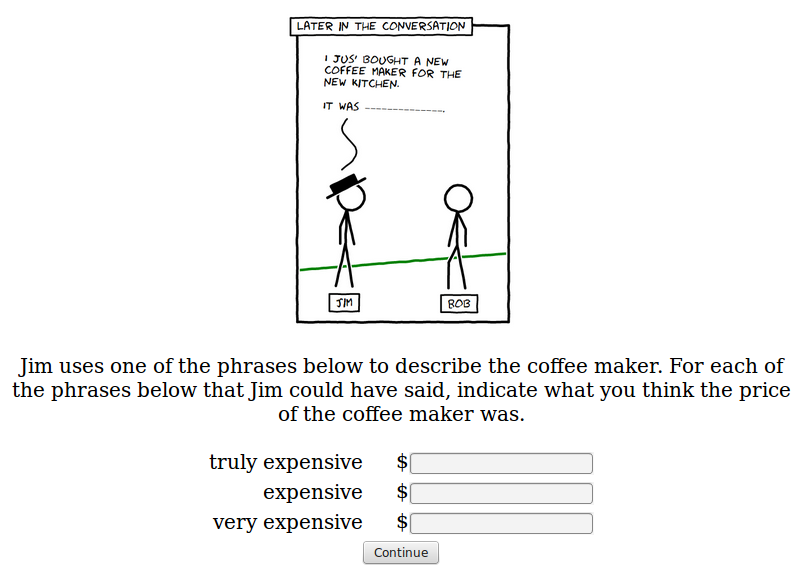
\includegraphics[width=0.4\textwidth]{analysis_files_for_writeup/images/exp3-q.png}
\end{center}
\caption{Screenshot from Experiment 3 target question.} 
\label{exp3-q}
\end{figure}

\subsection{Results and Discussion}

We calculated the difference score between the each of the intensifiers and the bare adjective ``expensive''.
We compared this difference score for each of the intensifiers when the intensifier was the target intensifier (highly frequent) and when it was the control (normal English frequency, but no occurances in the training story).

If infrequency causes an intensifier to be stronger, then we would expect participants would infer that the word is more frequent in this dialect and consequently less strong.
The difference score for the target intensifier would then be lower than for the control intensifier.

% We found that participants did learn that the speaker's use of a word was much higher when it was a target than when it was a control (Fig~\ref{exp3-freq-plot}). In a linear regression with word type (target or control) as a fixed effect and random intercepts for word and participant, word type was a significant predictor of frequency (estimate=34.06, p=0.0405).

%In addition,
We found that when participants believed the speaker's use of a word was much higher, they believed the meaning the speaker intended to convey with the word was lower (Fig~\ref{exp3-price-plot}).
The difference between ``\emph{[intensifier]} expensive'' and ``expensive'' was less for the target intensifier than for the control intensifier.
In a linear gregression with word type as a fixed effect and random intercepts for word and participant, word type was a significant predictor of difference score (estimate=-31.39, p=0.0226).

\begin{figure}[ht]
\begin{center}
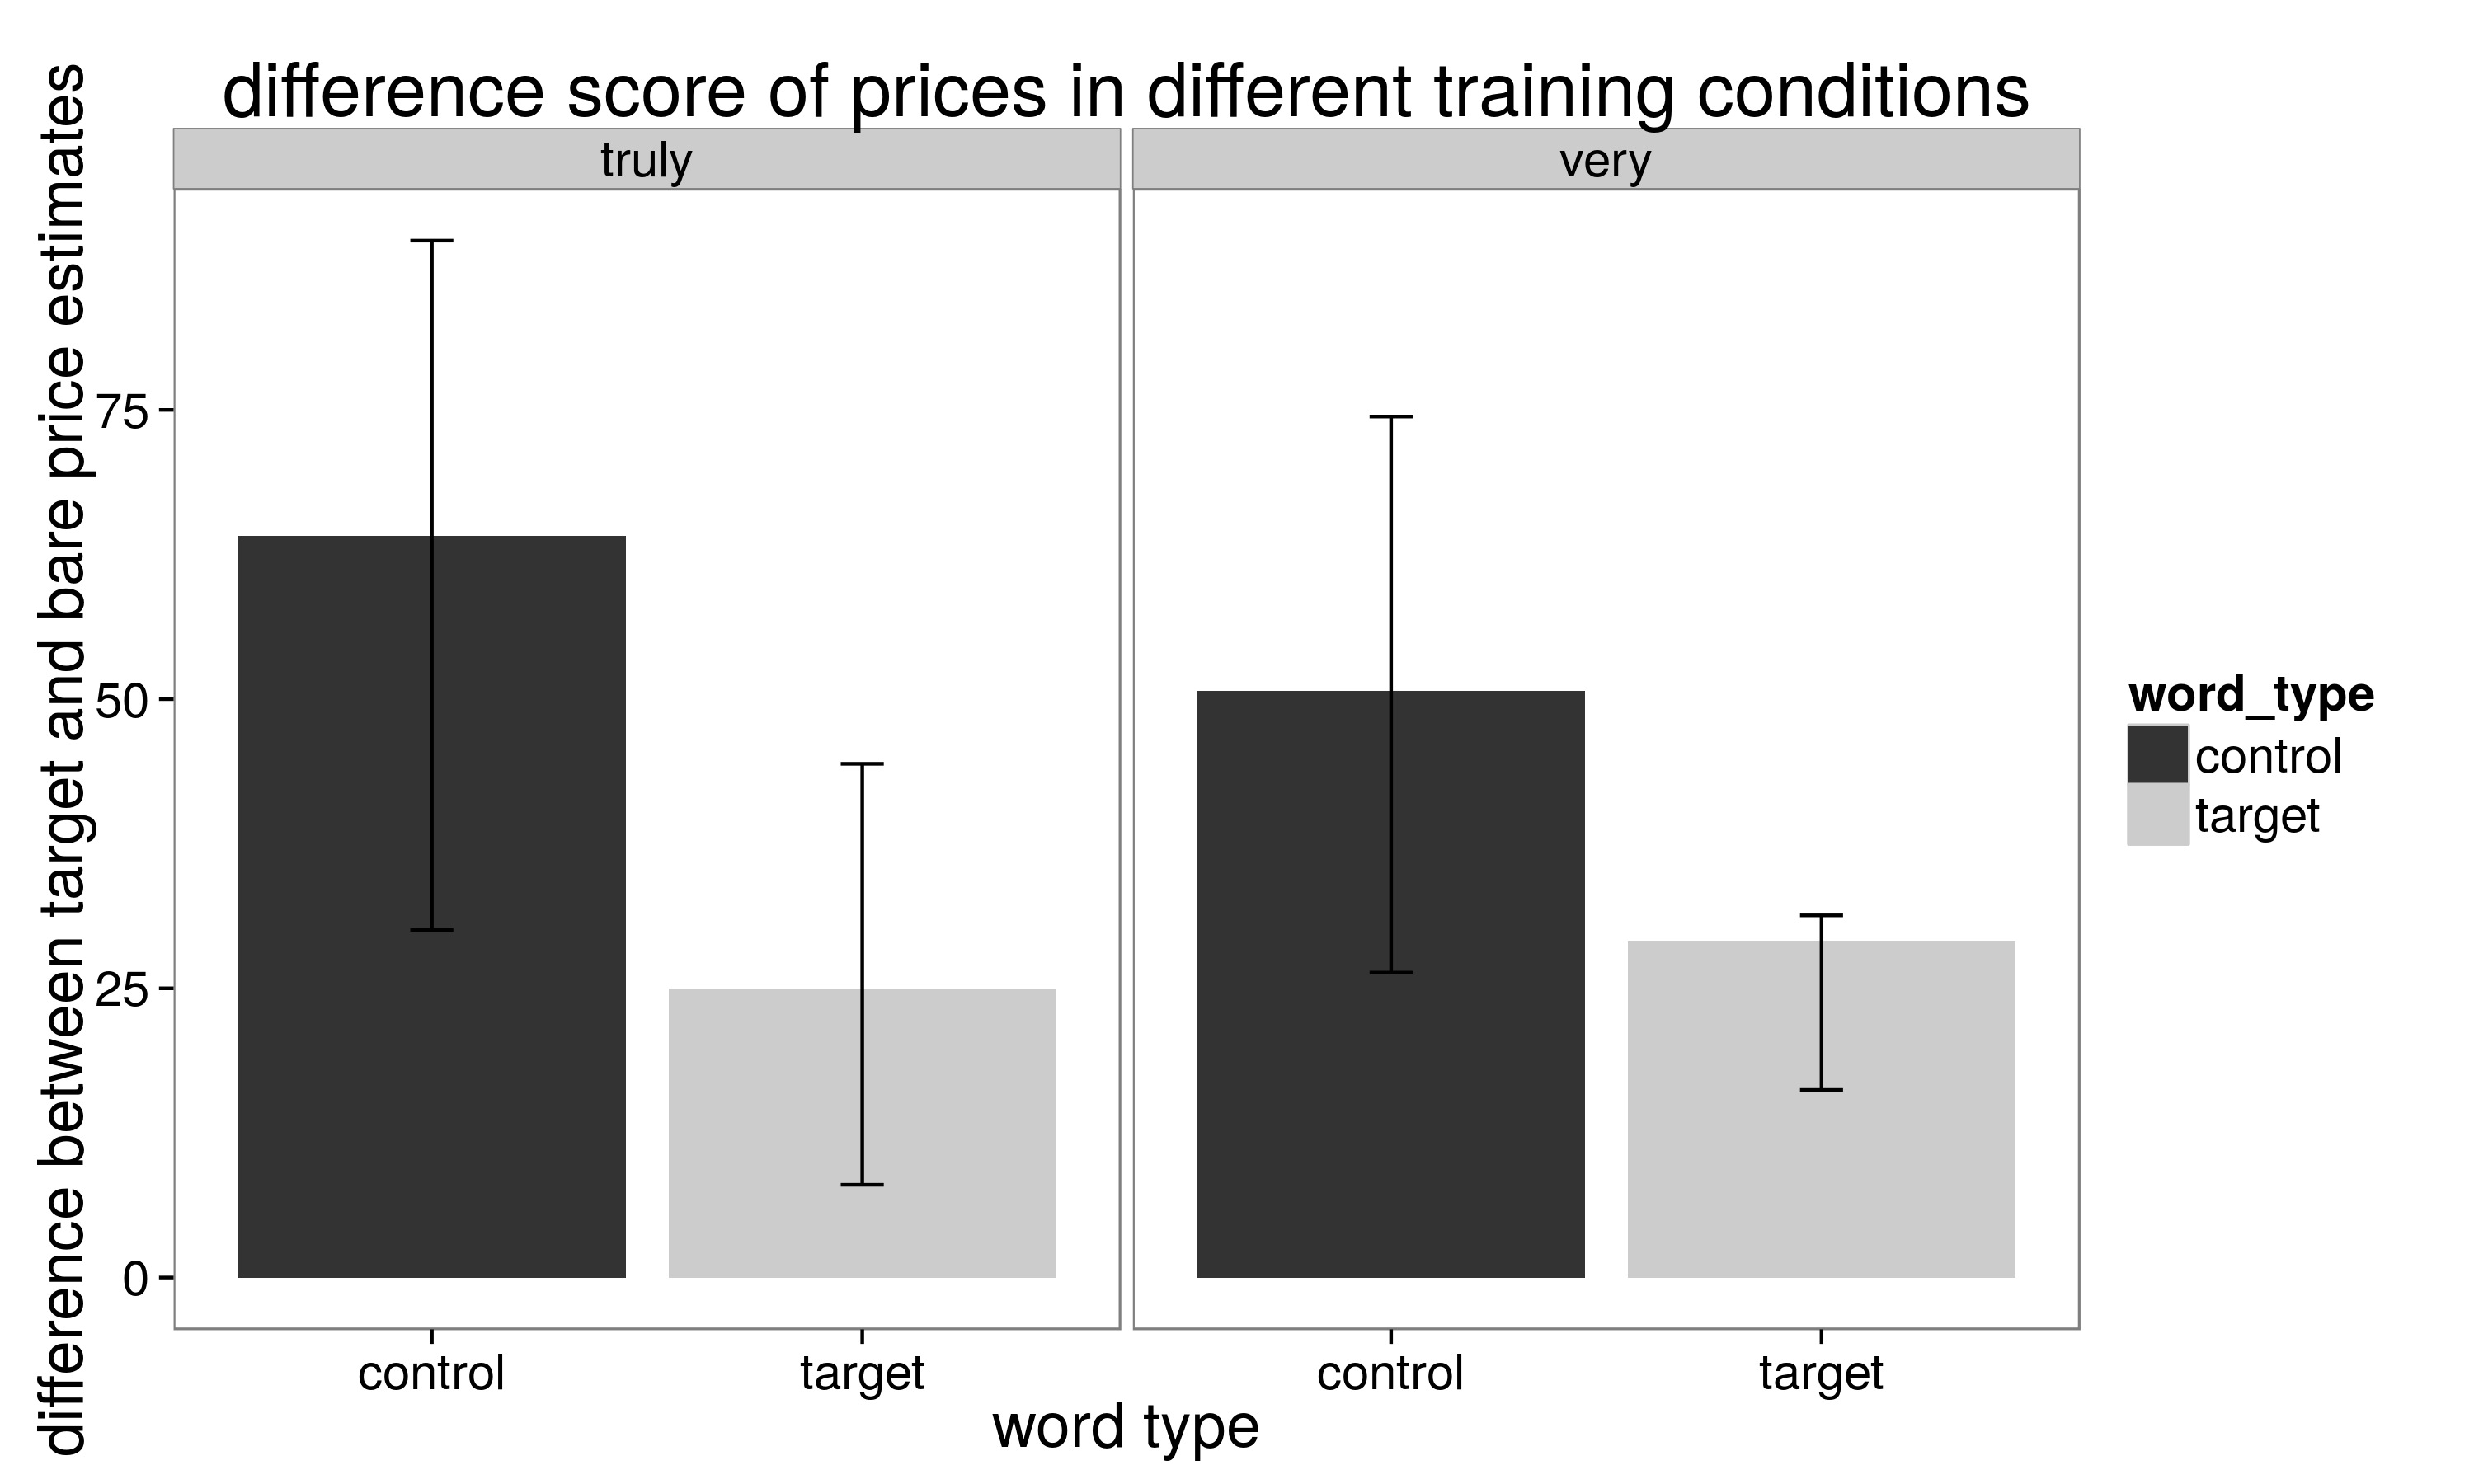
\includegraphics[width=0.48\textwidth]{analysis_files_for_writeup/images/exp3-price-plot.png}
\end{center}
\caption{Results of Experiment 3. Price estimate for intensifier is lower after the intensifier is repeated (target condition), showing that overuse within a dialect results in a less strong meaning.} 
\label{exp3-price-plot}
\end{figure}

In a linear regression with word type (target or control) as a fixed effect and random intercepts for word and participant, word type was a significant predictor of frequency (estimate=34.06, p=0.0405).

\todo[inline]{this is cool because we manipulated the frequency and the price estimate consequently dropped.}

%% gonna avoid this until i figure out about the dollar signs
% Individuals' estimates of frequency correlate with their estimates of price (Fig~\ref{exp3-scatterplot}, r=0.396, p=0.0169).
% 
% \begin{figure}[ht]
% \begin{center}
% 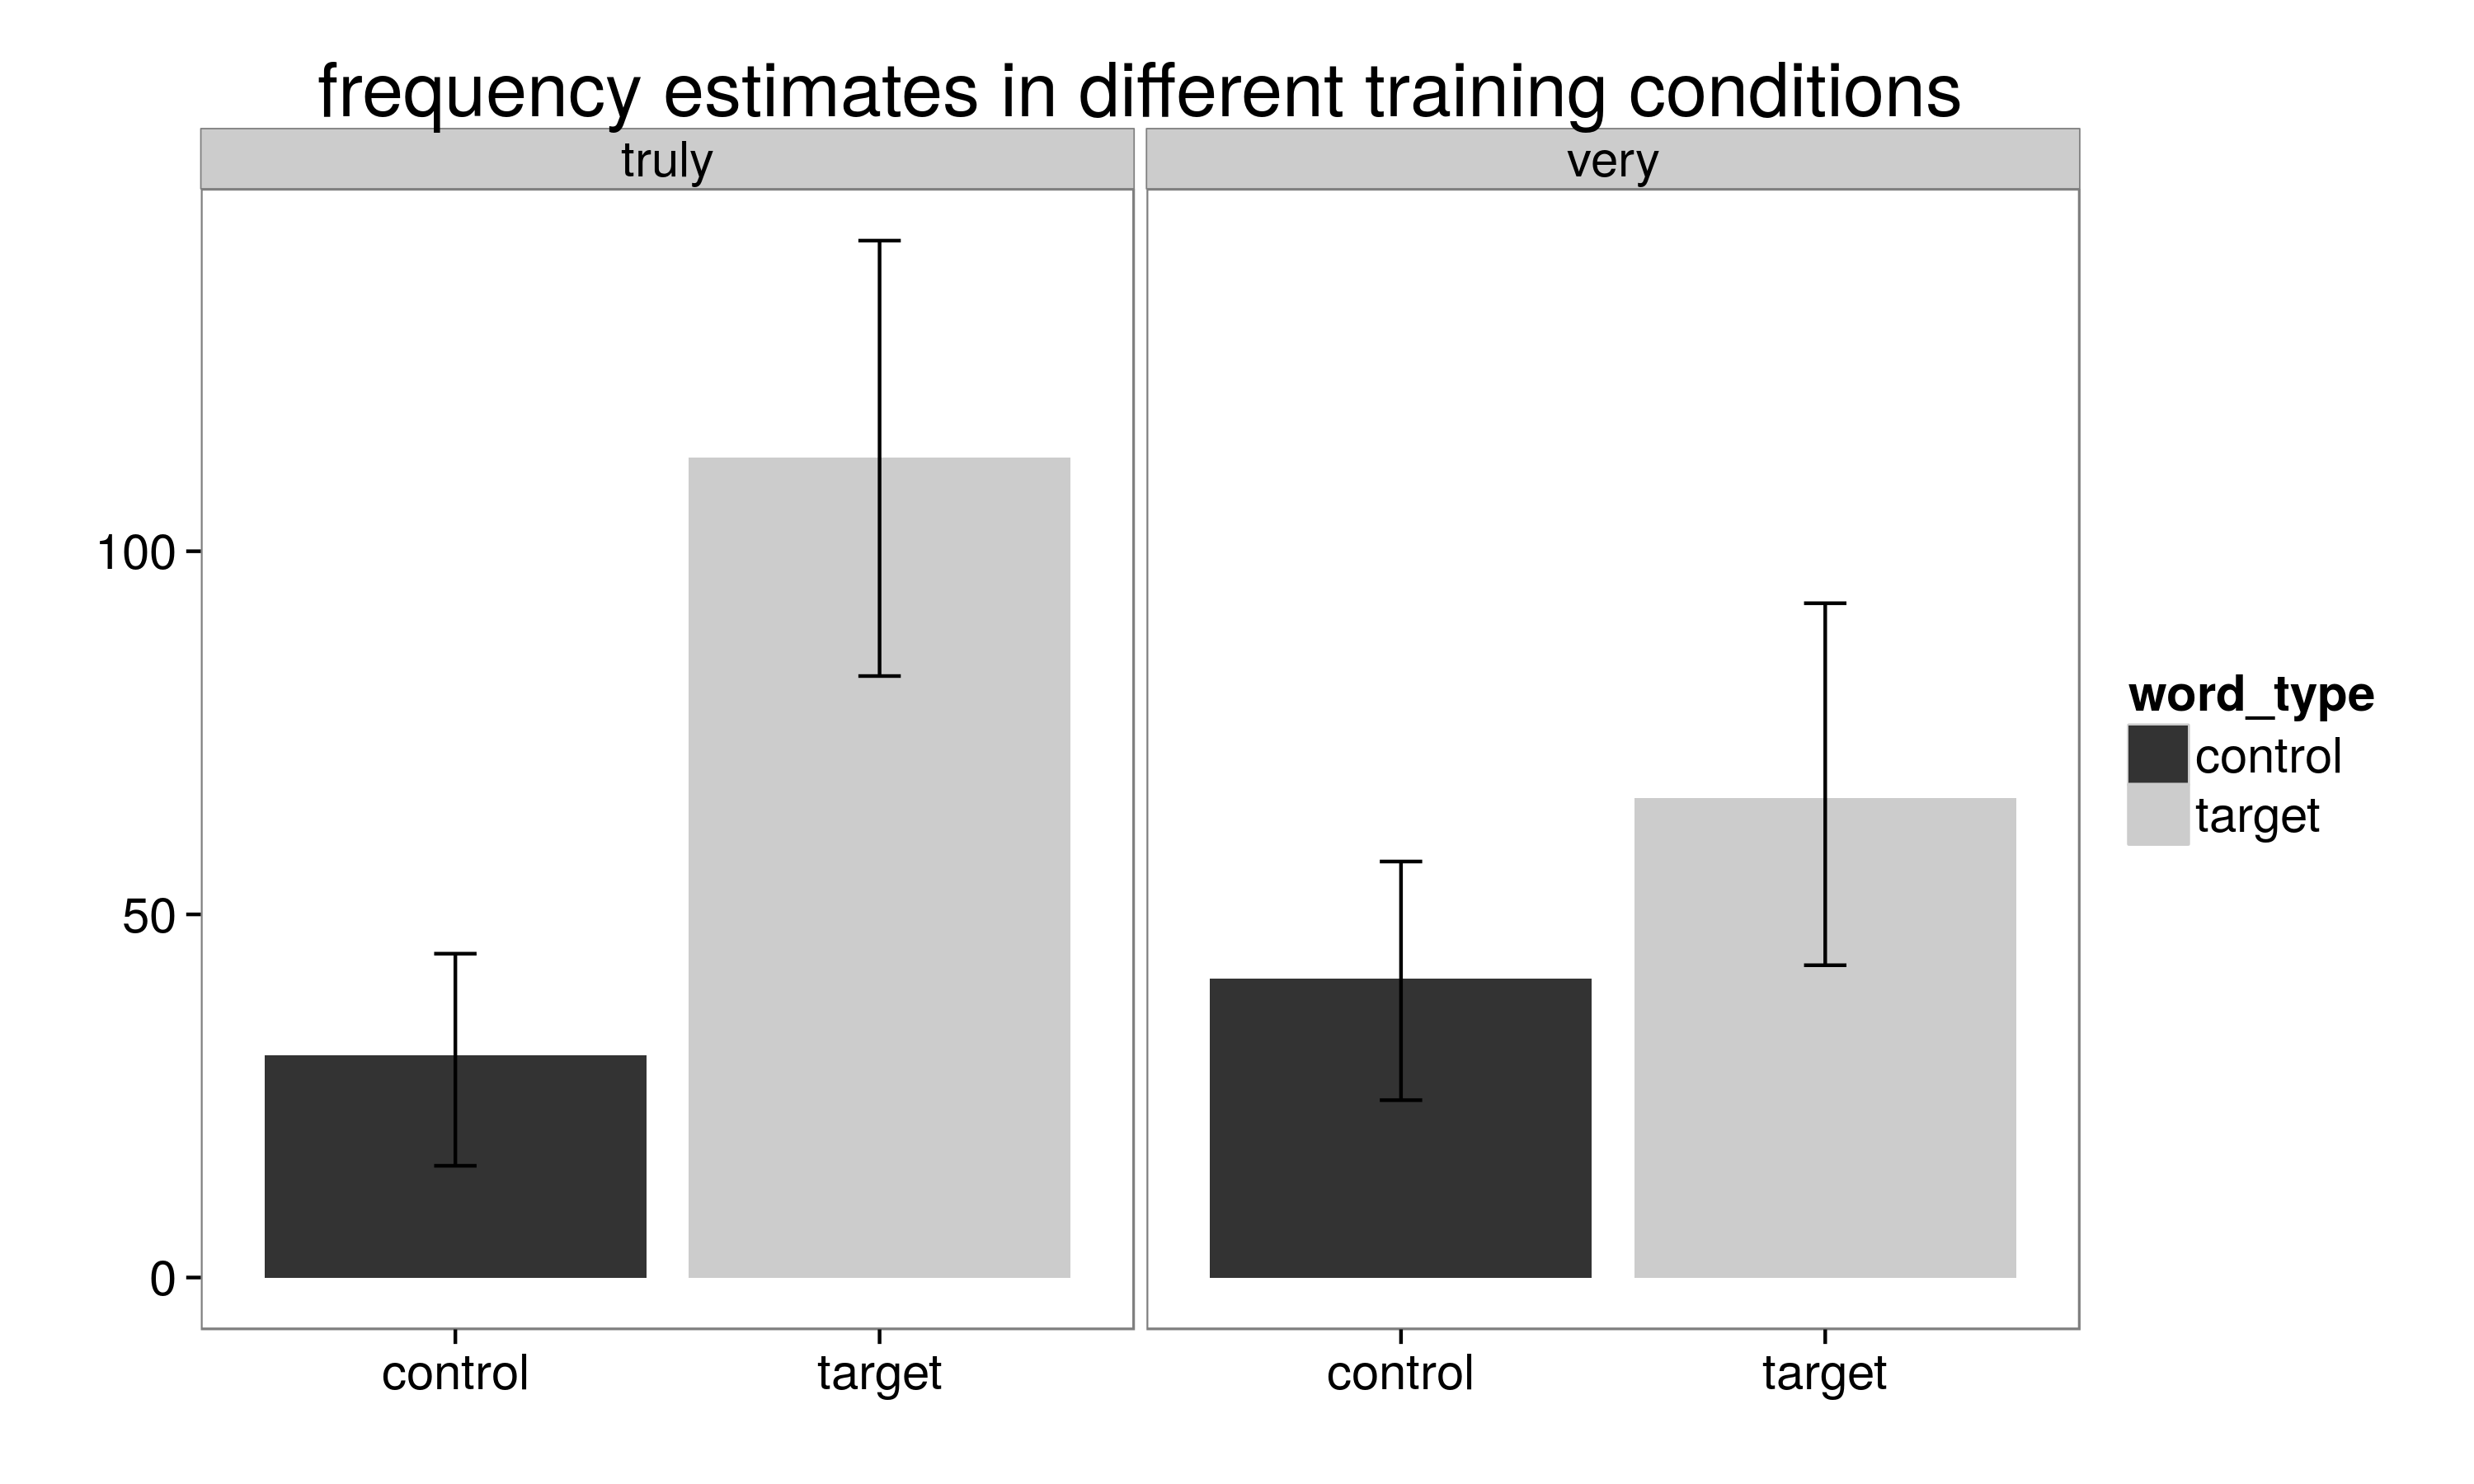
\includegraphics[width=0.48\textwidth]{analysis_files_for_writeup/images/exp3-freq-plot}
% \end{center}
% \caption{Results of Experiment 3. Intensifier is given a higher frequency estimate when it is target than when it is control, showing that participants learned a new frequency for that intensifier from the training.} 
% \label{exp3-freq-plot}
% \end{figure}
% \begin{figure}[ht]
% \begin{center}
% 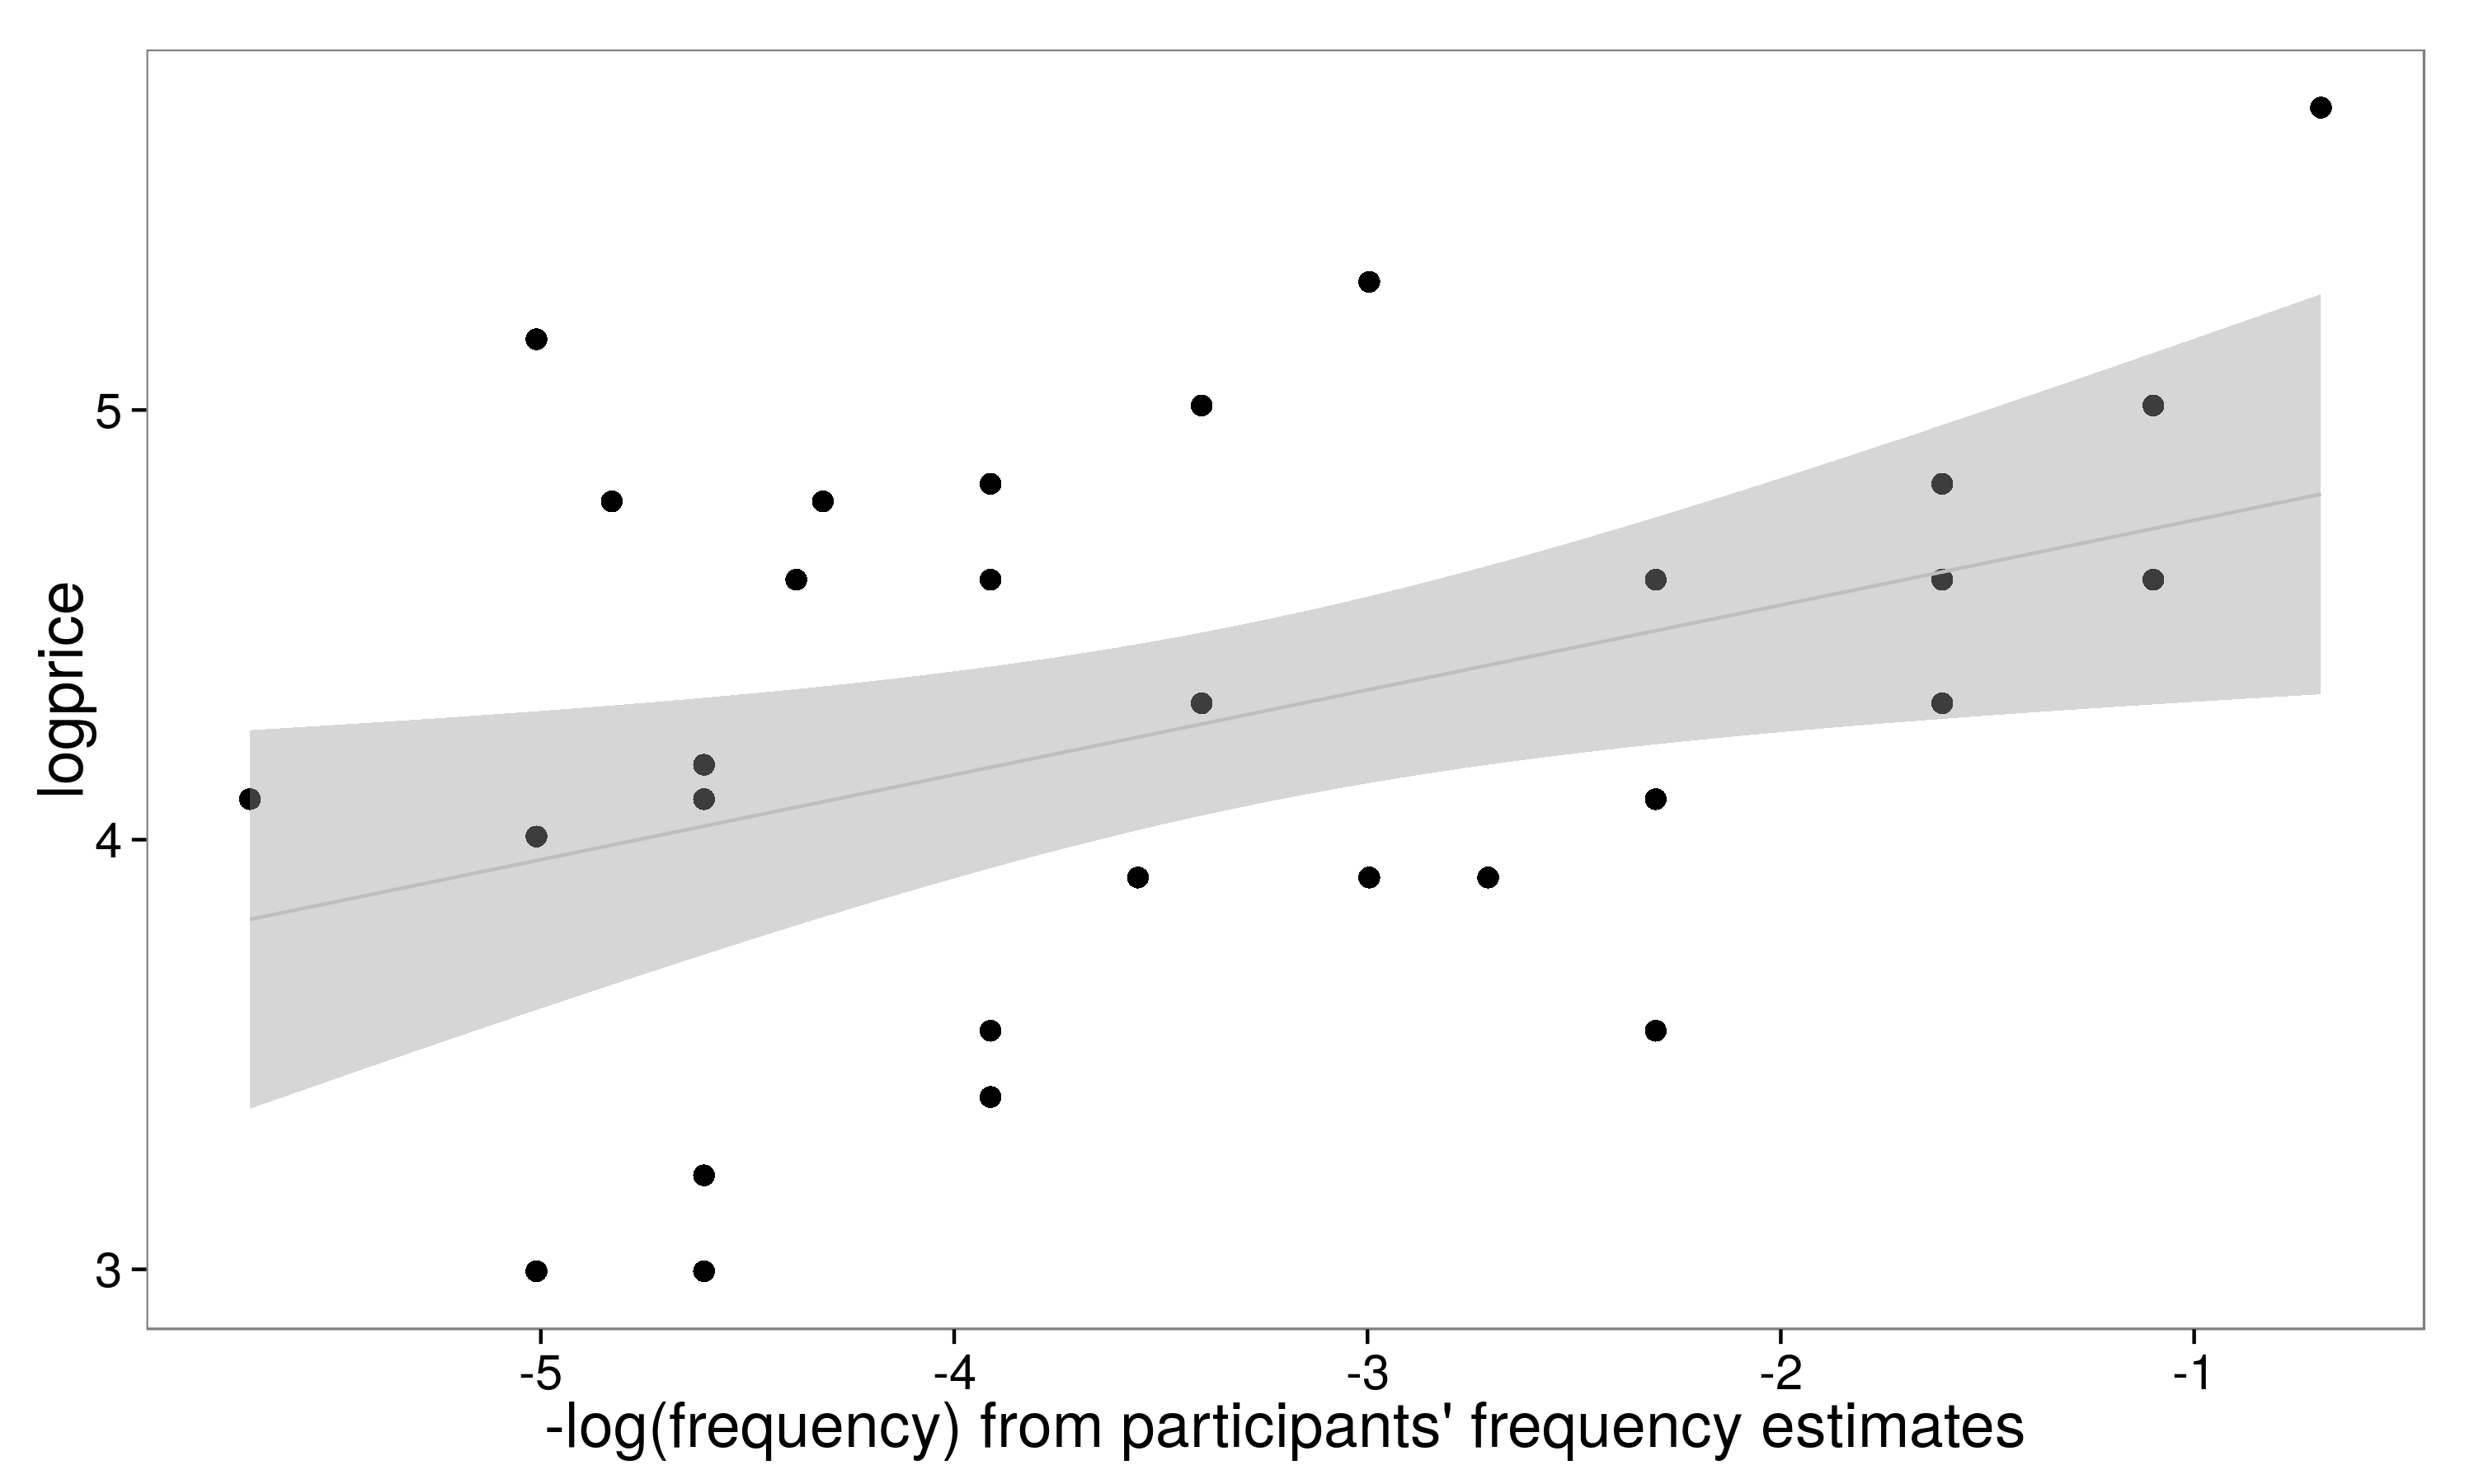
\includegraphics[width=0.48\textwidth]{analysis_files_for_writeup/images/exp3-scatterplot.png}
% \end{center}
% \caption{Results of Experiment 3. As participants' frequency estimates increase, their price estimates decrease.} 
% \label{exp3-scatterplot}
% \end{figure}

%do we have any way of estimating how much of an intensifier's meaning is determined by freq and syll? i'm not exactly sure how we would do this... maybe something like residual information not accounted for?

\section{Discussion}

%in general discussion / conclusion should address again the thing from the intro, also talk about other aspects of meaning (eg affect), issues with our results, and some future directions.

\todo[inline]{conclusion}

\section{Acknowledgments}

\nocite{web1t5gram}
\nocite{lewis}

\bibliographystyle{apacite}

\setlength{\bibleftmargin}{.125in}
\setlength{\bibindent}{-\bibleftmargin}

\bibliography{intensifiers}

\end{document}
